\ifdefined\inMainDoc\else
\documentclass[12pt,a4paper]{article}
% ================================================================
%  PRÉAMBULE COMMUN - ANNALES CORRIGÉES
%  Université de Kara - FaST - Licence Fondamentale MPC
%  Design optimisé impression noir et blanc
% ================================================================

% -- ENCODAGE & LANGUE --
\usepackage[utf8]{inputenc}
\usepackage[T1]{fontenc}
\usepackage[french]{babel}
\usepackage{lmodern}
\usepackage{microtype}

% -- MISE EN PAGE --
\usepackage[a4paper, top=2.8cm, bottom=2.5cm, left=2.5cm, right=2.5cm, headheight=14pt]{geometry}
\usepackage{setspace}
\setstretch{1.2}
\usepackage{parskip}
\setlength{\parindent}{1.2em}
\setlength{\parskip}{4pt}

% -- MATHS --
\usepackage{amsmath, amssymb, mathtools, amsthm}
\usepackage{mathrsfs}
\usepackage{dsfont}
\usepackage{bm}
\usepackage{cancel}
\usepackage{textcomp}
% Définition de \oiint (intégrale de surface fermée) sans package supplémentaire
\newcommand{\oiint}{\mathop{\iint\!\!\!\!\!\!\!\bigcirc}\limits}

% -- PHYSIQUE & CHIMIE --
\usepackage{physics}
\usepackage{siunitx}
% Lorsque physics est chargé, siunitx omet \qty. On le restaure ici :
\AtBeginDocument{\RenewCommandCopy\qty\SI}
\sisetup{locale = FR, detect-all, output-decimal-marker={,}}
% Commande de substitution pour les unités posant problème avec pdflatex
% (ohm, degreeCelsius, micro, angstrom, percent utilisent des caractères non-ASCII)
\newcommand{\qtyohm}[1]{\ensuremath{\num{#1}\,\Omega}}
\newcommand{\qtydegc}[1]{\ensuremath{\num{#1}\,{}^\circ\text{C}}}
\newcommand{\qtyangstrom}[1]{\ensuremath{\num{#1}\,\text{\AA}}}
\newcommand{\qtypercent}[1]{\ensuremath{\num{#1}\,\%}}
\newcommand{\qtyum}[1]{\ensuremath{\num{#1}\,\mu\text{m}}}
\usepackage[version=4]{mhchem}

% -- GRAPHISMES --
\usepackage{graphicx}
\usepackage{float}
\usepackage{caption}
\usepackage{subcaption}
\usepackage{wrapfig}
\usepackage{tikz}
\usetikzlibrary{calc, arrows.meta, patterns, shapes.geometric}
\usepackage{pgfplots}
\pgfplotsset{compat=1.18}

% -- TABLEAUX --
\usepackage{booktabs}
\usepackage{array}
\usepackage{tabularx}
\usepackage{multirow}

% -- LISTES --
\usepackage{enumitem}
\setlist[enumerate]{topsep=3pt, itemsep=2pt, parsep=0pt}
\setlist[itemize]{topsep=3pt, itemsep=2pt, parsep=0pt, label={.}}

% -- BOÎTES (noir et blanc) --
\usepackage{mdframed}
\usepackage{tcolorbox}
\tcbuselibrary{skins, breakable, theorems}

% Boîte EXERCICE : encadré avec filet épais, fond blanc
\newmdenv[
  linewidth=1.2pt,
  linecolor=black,
  roundcorner=3pt,
  skipabove=10pt,
  skipbelow=6pt,
  innertopmargin=8pt,
  innerbottommargin=8pt,
  innerleftmargin=10pt,
  innerrightmargin=10pt,
  backgroundcolor=white,
  frametitle={\bfseries\small Exercice},
  frametitlealignment=\raggedright,
  frametitleaboveskip=4pt,
  frametitlebelowskip=4pt,
]{boiteexercice}

% Boîte CORRIGÉ : fond gris très clair + filet fin
\newmdenv[
  linewidth=0.6pt,
  linecolor=black,
  leftline=true,
  rightline=false,
  topline=false,
  bottomline=false,
  linecolor=black,
  innerleftmargin=12pt,
  innerrightmargin=8pt,
  innertopmargin=6pt,
  innerbottommargin=6pt,
  backgroundcolor=gray!8,
  skipabove=4pt,
  skipbelow=8pt,
]{boitecorrige}

% Boîte RÉSUMÉ DE COURS : double encadré
\newmdenv[
  linewidth=0.8pt,
  linecolor=black,
  roundcorner=2pt,
  backgroundcolor=gray!12,
  innertopmargin=10pt,
  innerbottommargin=10pt,
  innerleftmargin=12pt,
  innerrightmargin=12pt,
  skipabove=12pt,
  skipbelow=8pt,
]{boiteresume}

% Boîte ATTENTION/REMARQUE : barre gauche épaisse
\newmdenv[
  leftline=true,
  rightline=false,
  topline=false,
  bottomline=false,
  linewidth=3pt,
  linecolor=black,
  backgroundcolor=gray!5,
  innerleftmargin=12pt,
  innerrightmargin=8pt,
  innertopmargin=5pt,
  innerbottommargin=5pt,
  skipabove=6pt,
  skipbelow=6pt,
]{boiteremarque}

% -- DIFFICULTÉ DES EXERCICES --
\newcommand{\facile}{$\star$}
\newcommand{\moyen}{$\star\!\star$}
\newcommand{\difficile}{$\star\!\star\!\star$}
\newcommand{\niveau}[1]{\hfill\textbf{#1}\hspace{2pt}}

% -- EN-TÊTES ET PIEDS DE PAGE --
\usepackage{fancyhdr}
\pagestyle{fancy}
\fancyhf{}
\renewcommand{\headrulewidth}{0.5pt}
\renewcommand{\footrulewidth}{0.3pt}

% -- HYPERLIENS --
\usepackage[hidelinks]{hyperref}
\hypersetup{
    colorlinks=false,
    pdftitle={Annale Corrigée - Licence MPC - Université de Kara}
}

% -- TITRES --
\usepackage{titlesec}
\titleformat{\section}{\Large\bfseries}{\thesection.}{0.8em}{}[\vspace{2pt}\hrule\vspace{4pt}]
\titleformat{\subsection}{\large\bfseries}{\thesubsection.}{0.7em}{}
\titleformat{\subsubsection}{\normalsize\bfseries}{\thesubsubsection.}{0.6em}{}

% -- THÉORÈMES --
\theoremstyle{definition}
\newtheorem{defn}{Définition}[section]
\newtheorem{prop}{Propriété}[section]
\newtheorem{thm}{Théorème}[section]
\newtheorem{corol}{Corollaire}[section]
\newtheorem{exemple}{Exemple}[section]

% -- COMMANDES MATHÉMATIQUES UTILES --
\newcommand{\vect}[1]{\overrightarrow{#1}}
\newcommand{\R}{\mathbb{R}}
\newcommand{\N}{\mathbb{N}}
\newcommand{\Z}{\mathbb{Z}}
\newcommand{\C}{\mathbb{C}}
\renewcommand{\d}{\mathrm{d}}
\newcommand{\deriv}[2]{\dfrac{\d #1}{\d #2}}
\newcommand{\dpart}[2]{\dfrac{\partial #1}{\partial #2}}
\newcommand{\rot}{\overrightarrow{\mathrm{rot}}\,}
\renewcommand{\div}{\mathrm{div}\,}
\renewcommand{\grad}{\overrightarrow{\mathrm{grad}}\,}
\newcommand{\e}{\mathrm{e}}
\newcommand{\ii}{\mathrm{i}}
\renewcommand{\Tr}{\mathrm{Tr}}

% Numérotation des équations par section
\numberwithin{equation}{section}

% -- RÉSULTATS ENCADRÉS --
\newcommand{\res}[1]{\[\boxed{#1}\]}

% -- REMARQUE INLINE --
\newcommand{\rmq}[1]{\begin{boiteremarque}\textbf{Remarque.} #1\end{boiteremarque}}

% -- MISE EN VALEUR DU RÉSULTAT FINAL --
\newcommand{\reponse}[1]{%
  \begin{center}
    \fbox{\begin{minipage}{0.92\textwidth}\centering #1\end{minipage}}
  \end{center}%
}


% En-têtes et pieds de page
\lhead{\textbf{Probabilités et Statistiques} - Licence 2}
\rhead{Université de Kara - FaST}
\cfoot{\thepage}
\lfoot{\textit{Licence Fondamentale MPC}}
\rfoot{\textit{Annales corrigées}}

\begin{document}
\fi

\begin{center}
  {\LARGE\bfseries Probabilités et Statistiques}\\[6pt]
  {\large Licence 2 - Mathématiques, Physique, Chimie}\\[4pt]
  {\normalsize Université de Kara - Faculté des Sciences et Techniques}
\end{center}

\vspace{8pt}
\hrule
\vspace{12pt}

% ================================================================
\section{Résumé de cours}
% ================================================================

\begin{boiteresume}
\textbf{1. Dénombrement}

Soit $n, k \in \mathbb{N}$ avec $k \leq n$.
\begin{itemize}
  \item \textbf{Arrangements} (ordre compte, sans répétition) : $A_n^k = \dfrac{n!}{(n-k)!}$
  \item \textbf{Permutations} de $n$ éléments : $P_n = n!$
  \item \textbf{Combinaisons} (ordre ne compte pas) : $\dbinom{n}{k} = \dfrac{n!}{k!\,(n-k)!}$
  \item \textbf{Formule de Pascal} : $\dbinom{n}{k} + \dbinom{n}{k+1} = \dbinom{n+1}{k+1}$
\end{itemize}

\medskip
\textbf{2. Probabilités - Axiomes de Kolmogorov}

Un espace de probabilité $(\Omega, \mathcal{A}, P)$ vérifie :
\begin{itemize}
  \item $P(\Omega) = 1$ et $P(A) \geq 0$ pour tout événement $A$.
  \item Additivité : si $A \cap B = \emptyset$ alors $P(A \cup B) = P(A) + P(B)$.
  \item $P(\bar{A}) = 1 - P(A)$.
\end{itemize}

\textbf{Probabilité conditionnelle} : $P(A \mid B) = \dfrac{P(A \cap B)}{P(B)}$ pour $P(B) > 0$.

\textbf{Formule des probabilités totales} : si $(A_i)$ est une partition de $\Omega$,
\[
P(B) = \sum_{i} P(B \mid A_i)\,P(A_i).
\]

\textbf{Théorème de Bayes} :
\[
P(A_i \mid B) = \frac{P(B \mid A_i)\,P(A_i)}{\displaystyle\sum_{j} P(B \mid A_j)\,P(A_j)}.
\]

\textbf{Indépendance} : $A$ et $B$ sont indépendants si et seulement si $P(A \cap B) = P(A)\,P(B)$.

\medskip
\textbf{3. Variables aléatoires discrètes}

Pour $X$ à valeurs dans $\{x_1, x_2, \ldots\}$ :
\[
\mathbb{E}(X) = \sum_i x_i\,P(X=x_i), \qquad
V(X) = \mathbb{E}(X^2) - [\mathbb{E}(X)]^2, \qquad
\sigma(X) = \sqrt{V(X)}.
\]

\begin{itemize}
  \item \textbf{Loi binomiale} $\mathcal{B}(n,p)$ : $P(X=k) = \dbinom{n}{k} p^k (1-p)^{n-k}$, $\mathbb{E}(X)=np$, $V(X)=np(1-p)$.
  \item \textbf{Loi de Poisson} $\mathcal{P}(\lambda)$ : $P(X=k) = \dfrac{\lambda^k}{k!}\,\mathrm{e}^{-\lambda}$, $\mathbb{E}(X)=\lambda$, $V(X)=\lambda$.
\end{itemize}

\medskip
\textbf{4. Variables aléatoires continues}

Densité $f \geq 0$ avec $\displaystyle\int_{-\infty}^{+\infty} f(x)\,\d x = 1$.
\[
\mathbb{E}(X) = \int x\,f(x)\,\mathrm{d}x, \qquad
V(X) = \int x^2 f(x)\,\mathrm{d}x - [\mathbb{E}(X)]^2.
\]

\begin{itemize}
  \item \textbf{Loi uniforme} $\mathcal{U}([a,b])$ : $f(x)=\dfrac{1}{b-a}$ sur $[a,b]$, $\mathbb{E}(X)=\dfrac{a+b}{2}$, $V(X)=\dfrac{(b-a)^2}{12}$.
  \item \textbf{Loi exponentielle} $\mathcal{E}(\lambda)$ : $f(x)=\lambda\,\mathrm{e}^{-\lambda x}$ pour $x\geq 0$, $\mathbb{E}(X)=\dfrac{1}{\lambda}$, $V(X)=\dfrac{1}{\lambda^2}$.
  \item \textbf{Loi normale} $\mathcal{N}(m,\sigma^2)$ : $f(x)=\dfrac{1}{\sigma\sqrt{2\pi}}\,\mathrm{e}^{-\frac{(x-m)^2}{2\sigma^2}}$, $\mathbb{E}(X)=m$, $V(X)=\sigma^2$.
\end{itemize}

\medskip
\textbf{5. Statistiques descriptives}

Pour une série de valeurs $x_1, \ldots, x_n$ :
\[
\bar{x} = \frac{1}{n}\sum x_i, \quad
s^2 = \frac{1}{n}\sum x_i^2 - \bar{x}^2, \quad
s = \sqrt{s^2}.
\]
La \textbf{médiane} $M_e$ vérifie $F(M_e) = 0{,}5$. Le \textbf{mode} est la valeur (ou classe) de plus grande fréquence. Les \textbf{quartiles} $Q_1$, $Q_2$, $Q_3$ correspondent aux fréquences cumulées $0{,}25$, $0{,}5$, $0{,}75$.
\end{boiteresume}

% ================================================================
\section{Exercices corrigés}
% ================================================================

% ----------------------
\begin{boiteexercice}
\textbf{Exercice 1 - Dénombrement dans un jeu de cartes}\niveau{\facile}

On tire simultanément 5 cartes d'un jeu de 32 cartes. Combien de tirages différents peut-on obtenir :
\begin{enumerate}
  \item sans contrainte sur les cartes ;
  \item contenant 5 carreaux ou 5 piques ;
  \item contenant 2 carreaux et 3 piques ;
  \item contenant au moins un roi ;
  \item contenant au plus un roi ;
  \item contenant exactement 2 rois et exactement 3 piques.
\end{enumerate}
\end{boiteexercice}

\begin{boitecorrige}
\textbf{1.} Un tirage est une combinaison de 5 cartes parmi 32 :
\[
\binom{32}{5} = 201\,376 \text{ tirages.}
\]

\textbf{2.} Choisir 5 carreaux parmi 8 ou 5 piques parmi 8 (cas disjoints) :
\[
2 \times \binom{8}{5} = 2 \times 56 = 112 \text{ tirages.}
\]

\textbf{3.} Choisir 2 carreaux parmi 8 puis 3 piques parmi 8 :
\[
\binom{8}{2} \times \binom{8}{3} = 28 \times 56 = 1\,568 \text{ tirages.}
\]

\textbf{4.} Par complémentaire (aucun roi : choisir 5 cartes parmi les 28 non-rois) :
\[
\binom{32}{5} - \binom{28}{5} = 201\,376 - 98\,280 = 103\,096 \text{ tirages.}
\]

\textbf{5.} Tirages sans roi : $\binom{28}{5}$. Tirages avec exactement un roi : $4 \times \binom{28}{4}$.
\[
\binom{28}{5} + 4\binom{28}{4} = 98\,280 + 4 \times 20\,475 = 180\,180 \text{ tirages.}
\]

\textbf{6.} On distingue deux cas selon que le roi de pique est présent ou non.

Si le tirage ne contient pas le roi de pique : choisir 2 rois parmi les 3 autres, puis 3 piques parmi les 7 piques non-rois.
\[
\binom{3}{2} \times \binom{7}{3} = 3 \times 35 = 105 \text{ tirages.}
\]

Si le tirage contient le roi de pique : choisir 1 roi parmi les 3 autres, 2 piques non-rois parmi 7, puis 1 carte ni roi ni pique parmi $32 - 4 - 7 = 21$.
\[
3 \times \binom{7}{2} \times 21 = 3 \times 21 \times 21 = 1\,323 \text{ tirages.}
\]

Total : $105 + 1\,323 = 1\,428$ tirages.
\end{boitecorrige}

% ----------------------
\begin{boiteexercice}
\textbf{Exercice 2 - Probabilités conditionnelles et théorème de Bayes}\niveau{\moyen}

Une urne $U_1$ contient 4 jetons blancs et 3 noirs ; une urne $U_2$ contient 17 jetons blancs et 18 noirs.

\textbf{Partie 1.} On lance un dé cubique équilibré. Si 6 apparaît, on tire de $U_1$, sinon de $U_2$. On note $A$ : « on a obtenu 6 » et $B$ : « on tire un jeton blanc ».
\begin{itemize}
  \item[a.] Calculer $P(B)$.
  \item[b.] Sachant qu'on a tiré un jeton blanc, calculer $P(A \mid B)$.
  \item[c.] Sachant qu'on a tiré un jeton noir, calculer $P(\bar{A} \mid \bar{B})$.
\end{itemize}

\textbf{Partie 2.} On tire successivement et sans remise les 7 jetons de $U_1$. La variable $X$ prend la valeur $k$ si le premier jeton blanc apparaît au $k$-ième tirage. Donner la loi de $X$, puis calculer son espérance et son écart-type.
\end{boiteexercice}

\begin{boitecorrige}
\textbf{Partie 1.}

On a $P(A) = \tfrac{1}{6}$, $P(\bar{A}) = \tfrac{5}{6}$, $P(B \mid A) = \tfrac{4}{7}$, $P(B \mid \bar{A}) = \tfrac{17}{35}$.

\textbf{a.} Par la formule des probabilités totales :
\[
P(B) = P(B \mid A)\,P(A) + P(B \mid \bar{A})\,P(\bar{A})
= \frac{4}{7} \cdot \frac{1}{6} + \frac{17}{35} \cdot \frac{5}{6}
= \frac{4}{42} + \frac{85}{210} = \frac{20}{210} + \frac{85}{210} = \frac{1}{2}.
\]

\textbf{b.} Par Bayes :
\[
P(A \mid B) = \frac{P(B \mid A)\,P(A)}{P(B)} = \frac{\tfrac{4}{7} \times \tfrac{1}{6}}{\tfrac{1}{2}} = \frac{4}{21}.
\]

\textbf{c.} $P(\bar{B}) = 1 - P(B) = \tfrac{1}{2}$. $P(\bar{B} \mid \bar{A}) = \tfrac{18}{35}$.
\[
P(\bar{A} \mid \bar{B}) = \frac{P(\bar{B} \mid \bar{A})\,P(\bar{A})}{P(\bar{B})} = \frac{\tfrac{18}{35} \times \tfrac{5}{6}}{\tfrac{1}{2}} = \frac{6}{7}.
\]

\textbf{Partie 2.} $U_1$ contient 4 blancs et 3 noirs, 7 jetons en tout. $X$ prend ses valeurs dans $\{1, 2, 3, 4\}$.

\[
\begin{array}{|c|c|c|c|c|}
\hline
k & 1 & 2 & 3 & 4 \\
\hline
P(X=k) & \dfrac{4}{7} & \dfrac{2}{7} & \dfrac{4}{35} & \dfrac{1}{35} \\
\hline
\end{array}
\]

Vérification : $\tfrac{4}{7} + \tfrac{2}{7} + \tfrac{4}{35} + \tfrac{1}{35} = \tfrac{20+10+4+1}{35} = 1$.

\[
\mathbb{E}(X) = 1 \cdot \frac{4}{7} + 2 \cdot \frac{2}{7} + 3 \cdot \frac{4}{35} + 4 \cdot \frac{1}{35}
= \frac{20 + 20 + 12 + 4}{35} = \frac{56}{35} = \frac{8}{5}.
\]

\[
\mathbb{E}(X^2) = 1 \cdot \frac{4}{7} + 4 \cdot \frac{2}{7} + 9 \cdot \frac{4}{35} + 16 \cdot \frac{1}{35}
= \frac{20 + 40 + 36 + 16}{35} = \frac{112}{35} = \frac{16}{5}.
\]

\[
V(X) = \frac{16}{5} - \left(\frac{8}{5}\right)^2 = \frac{16}{5} - \frac{64}{25} = \frac{80 - 64}{25} = \frac{16}{25}.
\qquad \sigma(X) = \frac{4}{5} = 0{,}8.
\]
\end{boitecorrige}

% ----------------------
\begin{boiteexercice}
\textbf{Exercice 3 - Variables aléatoires discrètes, covariance}\niveau{\moyen}

Soit $X$ une variable aléatoire dont la loi est donnée par :
\[
\begin{array}{|c|c|c|c|c|c|}
\hline
k & -2 & -1 & 0 & 1 & 2 \\
\hline
P(X=k) & \dfrac{1}{6} & \dfrac{1}{4} & \dfrac{1}{6} & \dfrac{1}{4} & \dfrac{1}{6} \\
\hline
\end{array}
\]
On pose $Y = X^2$.
\begin{enumerate}
  \item Déterminer la loi de $Y$.
  \item $X$ et $Y$ sont-elles indépendantes ?
  \item Calculer $\mathrm{Cov}(X, Y)$. Que remarque-t-on ?
\end{enumerate}
\end{boiteexercice}

\begin{boitecorrige}
\textbf{1. Loi de $Y = X^2$.}

$Y$ prend les valeurs $0, 1, 4$.
\[
P(Y=0) = P(X=0) = \frac{1}{6}.
\]
\[
P(Y=1) = P(X=-1) + P(X=1) = \frac{1}{4} + \frac{1}{4} = \frac{1}{2}.
\]
\[
P(Y=4) = P(X=-2) + P(X=2) = \frac{1}{6} + \frac{1}{6} = \frac{1}{3}.
\]

\[
\begin{array}{|c|c|c|c|}
\hline
y & 0 & 1 & 4 \\
\hline
P(Y=y) & \dfrac{1}{6} & \dfrac{1}{2} & \dfrac{1}{3} \\
\hline
\end{array}
\]

\textbf{2. Indépendance.}

Si $X$ et $Y$ étaient indépendantes, on aurait $P(X=-1,\,Y=4) = P(X=-1)\cdot P(Y=4)$. Or $P(X=-1,\,Y=4) = 0$ (car $(-1)^2 = 1 \neq 4$), mais $P(X=-1)\cdot P(Y=4) = \tfrac{1}{4} \times \tfrac{1}{3} = \tfrac{1}{12} \neq 0$. Donc $X$ et $Y$ ne sont pas indépendantes.

\textbf{3. Covariance.}

\[
\mathbb{E}[X] = (-2)\cdot\frac{1}{6} + (-1)\cdot\frac{1}{4} + 0 + 1\cdot\frac{1}{4} + 2\cdot\frac{1}{6} = 0 \quad \text{(loi symétrique).}
\]
\[
\mathbb{E}[Y] = 0 \cdot \frac{1}{6} + 1 \cdot \frac{1}{2} + 4 \cdot \frac{1}{3} = \frac{1}{2} + \frac{4}{3} = \frac{11}{6}.
\]
\[
\mathbb{E}[XY] = \mathbb{E}[X^3] = (-2)^3 \cdot \frac{1}{6} + (-1)^3 \cdot \frac{1}{4} + 0 + 1^3 \cdot \frac{1}{4} + 2^3 \cdot \frac{1}{6} = 0.
\]
\[
\mathrm{Cov}(X,Y) = \mathbb{E}[XY] - \mathbb{E}[X]\,\mathbb{E}[Y] = 0 - 0 = 0.
\]

Remarque : la covariance nulle ne suffit pas à établir l'indépendance. Ici, $X$ et $Y$ sont non corrélées mais non indépendantes.
\end{boitecorrige}

% ----------------------
\begin{boiteexercice}
\textbf{Exercice 4 - Loi de Poisson et couple de variables aléatoires}\niveau{\difficile}

Soient $X$ et $Y$ des variables aléatoires à valeurs dans $\mathbb{N}$ telles que, pour tout $(i,j) \in \mathbb{N}^2$ :
\[
P\bigl([X=i] \cap [Y=j]\bigr) = \frac{\alpha}{2^{i+j}\,j!}.
\]
\begin{enumerate}
  \item Déterminer $\alpha$.
  \item Déterminer les lois marginales de $X$ et de $Y$.
  \item Calculer $\mathrm{Cov}(X,Y)$. $X$ et $Y$ sont-elles indépendantes ?
\end{enumerate}
\end{boiteexercice}

\begin{boitecorrige}
\textbf{1. Détermination de $\alpha$.}

La somme de toutes les probabilités doit être égale à 1 :
\[
\sum_{i=0}^{\infty}\sum_{j=0}^{\infty} \frac{\alpha}{2^{i+j}\,j!}
= \alpha \left(\sum_{i=0}^{\infty} \frac{1}{2^i}\right)\left(\sum_{j=0}^{\infty} \frac{1}{2^j\,j!}\right)
= \alpha \cdot \frac{1}{1-\tfrac{1}{2}} \cdot \mathrm{e}^{1/2}
= 2\alpha\,\mathrm{e}^{1/2} = 1.
\]
Donc $\alpha = \dfrac{1}{2\,\mathrm{e}^{1/2}} = \dfrac{\mathrm{e}^{-1/2}}{2}$.

\textbf{2. Lois marginales.}

Loi de $X$ :
\[
P(X=i) = \sum_{j=0}^{\infty} \frac{\alpha}{2^{i+j}\,j!}
= \frac{\alpha}{2^i}\,\mathrm{e}^{1/2} = \frac{\mathrm{e}^{-1/2}}{2} \cdot \frac{\mathrm{e}^{1/2}}{2^i} = \frac{1}{2^{i+1}}.
\]
C'est une loi géométrique sur $\mathbb{N}$ de paramètre $\tfrac{1}{2}$ (avec $i \geq 0$).

Loi de $Y$ :
\[
P(Y=j) = \sum_{i=0}^{\infty} \frac{\alpha}{2^{i+j}\,j!}
= \frac{\alpha}{2^j\,j!} \cdot 2 = \frac{\mathrm{e}^{-1/2}}{2^j\,j!}.
\]
En posant $\lambda = \tfrac{1}{2}$, on reconnaît $P(Y=j) = \dfrac{\mathrm{e}^{-\lambda}\,\lambda^j}{j!}$ : c'est une loi de Poisson $\mathcal{P}\!\left(\tfrac{1}{2}\right)$.

\textbf{3. Covariance.}

$\mathbb{E}(X) = \displaystyle\sum_{i=0}^{\infty} \frac{i}{2^{i+1}} = \frac{1}{2}\cdot\frac{1/(1-1/2)^2}{2} = 1$ (série arithmético-géométrique).

$\mathbb{E}(Y) = \lambda = \tfrac{1}{2}$ (espérance de $\mathcal{P}(\tfrac{1}{2})$).

\[
\mathbb{E}(XY) = \sum_{i,j} ij \cdot \frac{\alpha}{2^{i+j}\,j!}
= \alpha \left(\sum_i \frac{i}{2^i}\right)\!\left(\sum_j \frac{j}{2^j\,j!}\right)
= \alpha \cdot 2 \cdot \frac{\mathrm{e}^{1/2}}{4} = \frac{1}{2}.
\]

\[
\mathrm{Cov}(X,Y) = \mathbb{E}(XY) - \mathbb{E}(X)\,\mathbb{E}(Y) = \frac{1}{2} - 1 \cdot \frac{1}{2} = 0.
\]

De plus, $P(X=i)\cdot P(Y=j) = \dfrac{1}{2^{i+1}} \cdot \dfrac{\mathrm{e}^{-1/2}}{2^j\,j!} = \dfrac{\mathrm{e}^{-1/2}}{2^{i+j+1}\,j!} = P(X=i,\,Y=j)$.

Donc $X$ et $Y$ sont indépendantes (et la covariance nulle en est la conséquence).
\end{boitecorrige}

% ----------------------
\begin{boiteexercice}
\textbf{Exercice 5 - Statistiques descriptives : loyers}\niveau{\moyen}

Une enquête sur les loyers annuels (en milliers de francs) d'un quartier donne :

\[
\begin{array}{|c|c|}
\hline
\text{Classe de loyer} & \text{Effectif} \\
\hline
{[4\,;\,6[} & 20 \\
{[6\,;\,8[} & 40 \\
{[8\,;\,10[} & 80 \\
{[10\,;\,15[} & 30 \\
{[15\,;\,20[} & 20 \\
{[20\,;\,30[} & 10 \\
\hline
\end{array}
\]

\begin{enumerate}
  \item Compléter le tableau (valeur centrale, fréquence, fréquences cumulées, densité).
  \item Déterminer la moyenne, le mode et les quartiles $Q_1$, $Q_2$, $Q_3$.
  \item Calculer l'étendue, l'écart-type et l'intervalle interquartile.
\end{enumerate}
\end{boiteexercice}

\begin{boitecorrige}
L'effectif total est $n = 200$.

\textbf{1. Tableau complété.}

\[
\begin{array}{|c|c|c|c|c|c|}
\hline
\text{Classe} & x_i & n_i & N_i & f_i & d_i \\
\hline
{[4;6[}   & 5  & 20  & 20  & 0{,}10 & 10 \\
{[6;8[}   & 7  & 40  & 60  & 0{,}20 & 20 \\
{[8;10[}  & 9  & 80  & 140 & 0{,}40 & 40 \\
{[10;15[} & 12{,}5 & 30 & 170 & 0{,}15 & 6 \\
{[15;20[} & 17{,}5 & 20 & 190 & 0{,}10 & 4 \\
{[20;30[} & 25 & 10  & 200 & 0{,}05 & 1 \\
\hline
\end{array}
\]

\textbf{2. Moyenne, mode, quartiles.}

\[
\bar{x} = \sum f_i\,x_i = 0{,}10\times5 + 0{,}20\times7 + 0{,}40\times9 + 0{,}15\times12{,}5 + 0{,}10\times17{,}5 + 0{,}05\times25 = 10{,}375.
\]

La classe modale est $[8\,;\,10[$ (densité maximale $= 40$).
\[
M_o = 8 + \frac{40-20}{(40-20)+(40-30)} \times 2 = 8 + \frac{20}{30} \times 2 \approx 9{,}33.
\]

Pour les quartiles, on utilise $Q_p = a_i + (a_{i+1}-a_i)\cdot\dfrac{p\,n/4 - N_{i-1}}{n_i}$ :
\[
Q_1 : F = 0{,}25,\text{ classe } [8;10[. \quad Q_1 = 8 + 2 \cdot \frac{0{,}25 - 0{,}30}{0{,}40} = 7{,}5 \times 10^3.
\]
\[
Q_2 : F = 0{,}50,\text{ classe } [8;10[. \quad Q_2 = 8 + 2 \cdot \frac{0{,}50 - 0{,}30}{0{,}40} = 9{,}0 \times 10^3.
\]
\[
Q_3 : F = 0{,}75,\text{ classe } [10;15[. \quad Q_3 = 10 + 5 \cdot \frac{0{,}75 - 0{,}70}{0{,}15} \approx 11{,}67 \times 10^3.
\]

\textbf{3. Dispersion.}

Étendue : $W = (30-4) \times 1000 = 26\,000$ F.

Intervalle interquartile : $\mathrm{IQ} = Q_3 - Q_1 = (11\,667 - 7\,500) = 4\,167$ F.

\[
\sigma^2 = \sum f_i\,x_i^2 - \bar{x}^2, \qquad \sigma \approx 5{,}43 \times 10^3 \text{ F}.
\]
\end{boitecorrige}

% ----------------------
\begin{boiteexercice}
\textbf{Exercice 6 - Régression linéaire}\niveau{\moyen}

On dispose des données suivantes (5 points) :
\[
\begin{array}{c|ccccc}
x_i & 2 & 5 & 6 & 10 & 12 \\
\hline
y_i & 83 & 70 & 70 & 54 & 49
\end{array}
\]
\begin{enumerate}
  \item Calculer la covariance $\mathrm{Cov}(X,Y)$.
  \item Déterminer l'équation de la droite de régression $Y = aX + b$.
  \item Calculer le coefficient de corrélation linéaire $r$ et commenter.
\end{enumerate}
\end{boiteexercice}

\begin{boitecorrige}
$n = 5$.

\[
\bar{X} = \frac{2+5+6+10+12}{5} = 7, \qquad \bar{Y} = \frac{83+70+70+54+49}{5} = 65{,}2.
\]

\textbf{1.}
\[
\mathrm{Cov}(X,Y) = \frac{1}{n}\sum X_i Y_i - \bar{X}\,\bar{Y}
= \frac{\sum X_i Y_i}{5} - 7 \times 65{,}2.
\]
où $\sum X_i Y_i = 2\cdot83 + 5\cdot70 + 6\cdot70 + 10\cdot54 + 12\cdot49$.
\[
\frac{166 + 350 + 420 + 540 + 588}{5} = \frac{2064}{5} = 412{,}8.
\quad \mathrm{Cov}(X,Y) = 412{,}8 - 456{,}4 = -43{,}6.
\]

\textbf{2.}
\[
V(X) = \frac{1}{n}\sum X_i^2 - \bar{X}^2 = \frac{4+25+36+100+144}{5} - 49 = 61{,}8 - 49 = 12{,}8.
\]
\[
a = \frac{\mathrm{Cov}(X,Y)}{V(X)} = \frac{-43{,}6}{12{,}8} \approx -3{,}406, \qquad
b = \bar{Y} - a\bar{X} = 65{,}2 - (-3{,}406)\times 7 \approx 89.
\]
\[
\boxed{Y = -3{,}41\,X + 89.}
\]

\textbf{3.}
\[
V(Y) = \frac{83^2+70^2+70^2+54^2+49^2}{5} - 65{,}2^2 = 4\,257{,}2 - 4\,251{,}04 \approx 143{,}36.
\]
\[
r = \frac{\mathrm{Cov}(X,Y)}{\sqrt{V(X)\,V(Y)}} = \frac{-43{,}6}{\sqrt{12{,}8 \times 143{,}36}} \approx \frac{-43{,}6}{42{,}83} \approx -1{,}02 \approx -1.
\]

La valeur $r \approx -1$ indique une forte corrélation linéaire négative entre $X$ et $Y$ : quand le chiffre augmente, l'autre diminue de façon quasi proportionnelle.
\end{boitecorrige}

% ----------------------
\begin{boiteexercice}
\textbf{Exercice 7 - Loi normale}\niveau{\moyen}

Montrer que si $X \sim \mathcal{N}(0,1)$, alors $Z = \sigma X + m$ suit une loi $\mathcal{N}(m, \sigma^2)$.

Calculer ensuite $\mathbb{E}(Z)$ et $V(Z)$ directement à partir des propriétés de l'espérance et de la variance.
\end{boiteexercice}

\begin{boitecorrige}
\textbf{Calcul par transformation de la densité.}

La densité de $X \sim \mathcal{N}(0,1)$ est $f_X(x) = \dfrac{1}{\sqrt{2\pi}}\,\mathrm{e}^{-x^2/2}$.

On pose $Z = \sigma X + m$, donc $X = \dfrac{Z-m}{\sigma}$ et $\dfrac{\mathrm{d}x}{\mathrm{d}z} = \dfrac{1}{\sigma}$.

Par la formule de changement de variable :
\[
f_Z(z) = f_X\!\left(\frac{z-m}{\sigma}\right) \cdot \frac{1}{|\sigma|}
= \frac{1}{\sqrt{2\pi}}\,\mathrm{e}^{-\frac{(z-m)^2}{2\sigma^2}} \cdot \frac{1}{\sigma}
= \frac{1}{\sigma\sqrt{2\pi}}\,\mathrm{e}^{-\frac{(z-m)^2}{2\sigma^2}}.
\]

C'est bien la densité d'une loi $\mathcal{N}(m, \sigma^2)$.

\textbf{Par les propriétés de l'espérance et de la variance :}
\[
\mathbb{E}(Z) = \mathbb{E}(\sigma X + m) = \sigma\,\mathbb{E}(X) + m = \sigma \times 0 + m = m.
\]
\[
V(Z) = V(\sigma X + m) = \sigma^2\,V(X) = \sigma^2 \times 1 = \sigma^2.
\]

Ainsi $Z \sim \mathcal{N}(m, \sigma^2)$, ce qui confirme le résultat précédent.
\end{boitecorrige}

\section{Variables aléatoires discrètes et continues}

\subsection*{Exercice 8 - Variable aléatoire uniforme discrète \niveau{\facile}}

\begin{boiteexercice}
Soit $X$ une variable aléatoire de loi uniforme sur $X(\Omega) = \{-3; -2; 1; 4\}$.
\begin{enumerate}
  \item Donner la loi de $X$.
  \item Calculer $\mathbb{E}(X)$ et $V(X)$.
  \item On pose $Y = 2X+1$. Donner $Y(\Omega)$ et la loi de $Y$.
  \item Calculer $\mathbb{E}(Y)$ de deux façons différentes.
\end{enumerate}
\end{boiteexercice}

\begin{boitecorrige}
\textbf{1.} La loi uniforme sur 4 valeurs équiprobables :
\[
P(X=-3)=P(X=-2)=P(X=1)=P(X=4)=\frac{1}{4}
\]

\textbf{2.}
\[
\mathbb{E}(X) = \frac{1}{4}(-3-2+1+4) = \frac{0}{4} = 0
\]
\[
\mathbb{E}(X^2) = \frac{1}{4}(9+4+1+16) = \frac{30}{4} = 7{,}5 \quad\Rightarrow\quad V(X) = 7{,}5 - 0^2 = 7{,}5
\]

\textbf{3.} $Y(\Omega) = \{2(-3)+1, 2(-2)+1, 2(1)+1, 2(4)+1\} = \{-5, -3, 3, 9\}$. Comme $Y$ est une fonction bijective de $X$, chaque valeur a probabilité $1/4$.

\textbf{4.} \emph{Méthode 1 (linéarité de l'espérance)} : $\mathbb{E}(Y) = 2\mathbb{E}(X)+1 = 2\times0+1 = 1$.

\emph{Méthode 2 (calcul direct)} :
\[
\mathbb{E}(Y) = \frac{1}{4}(-5-3+3+9) = \frac{4}{4} = 1
\]
Les deux méthodes donnent $\mathbb{E}(Y) = 1$.
\end{boitecorrige}

\subsection*{Exercice 9 - Statistiques descriptives : loyers \niveau{\moyen}}

\begin{boiteexercice}
Une enquête sur les loyers annuels (en milliers de francs CFA) d'appartements donne :
\[
\begin{array}{|c|c|}
\hline
\text{Classe de loyer (×1000)} & \text{Effectif} \\
\hline
${[}4;6{[}$ & 20 \\
${[}6;8{[}$ & 40 \\
${[}8;10{[}$ & 80 \\
${[}10;15{[}$ & 30 \\
${[}15;20{[}$ & 20 \\
${[}20;30{[}$ & 10 \\
\hline
\end{array}
\]
\begin{enumerate}
  \item Calculer la moyenne, le mode, la médiane et les quartiles $Q_1$, $Q_3$.
  \item Calculer l'étendue, l'écart-type et l'intervalle interquartile.
\end{enumerate}
\end{boiteexercice}

\begin{boitecorrige}
L'effectif total est $n = 200$. Les valeurs centrales des classes sont : $5, 7, 9, 12{,}5, 17{,}5, 25$.

\textbf{1.} Moyenne :
\[
\bar{x} = \frac{1}{200}(20\times5 + 40\times7 + 80\times9 + 30\times12{,}5 + 20\times17{,}5 + 10\times25) = \frac{2075}{200} \approx 10{,}375 \text{ milliers}
\]
La classe modale est $[8;10[$ (plus grande densité $= 80/2 = 40$). Le mode vaut :
\[
M = 8 + \frac{(80-40)}{(80-40)+(80-30)}\times 2 \approx 8{,}89\text{ milliers}
\]
Les effectifs cumulés : $20, 60, 140, 170, 190, 200$. La médiane ($n/2 = 100$) est dans $[8;10[$ :
\[
\text{Médiane} = 8 + \frac{100-60}{80}\times 2 = 8 + 1 = 9\text{ milliers}
\]
$Q_1$ ($n/4=50$) dans $[6;8[$ : $Q_1 = 6 + \frac{50-20}{40}\times2 = 7{,}5$ milliers.

$Q_3$ ($3n/4=150$) dans $[10;15[$ : $Q_3 = 10 + \frac{150-140}{30}\times5 \approx 11{,}67$ milliers.

\textbf{2.} Étendue $= (30-4) = 26$ milliers. Intervalle interquartile $= Q_3-Q_1 \approx 4{,}17$ milliers.

Variance : $\sigma^2 = \frac{1}{200}\sum n_i x_i^2 - \bar{x}^2$. En calculant $\sum n_i x_i^2 = 20(25)+40(49)+80(81)+30(156{,}25)+20(306{,}25)+10(625) = 26\,037{,}5$, d'où $\sigma^2 = 130{,}19 - 107{,}64 \approx 22{,}55$, soit $\sigma \approx 4{,}75$ milliers.

\begin{center}
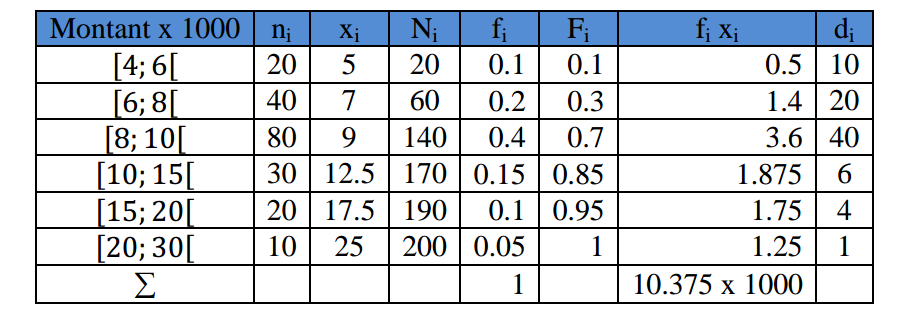
\includegraphics[width=0.85\textwidth]{images/probabilites/prob-015-000.png}\\[4pt]
{\small\itshape Tableau statistique complété (document original).}
\end{center}

\begin{center}

\includegraphics[width=0.85\textwidth]{images/probabilites/prob-015-001.png}\\[4pt]
{\small\itshape Histogramme des effectifs par classe de salaire (document original).}
\end{center}

\begin{center}
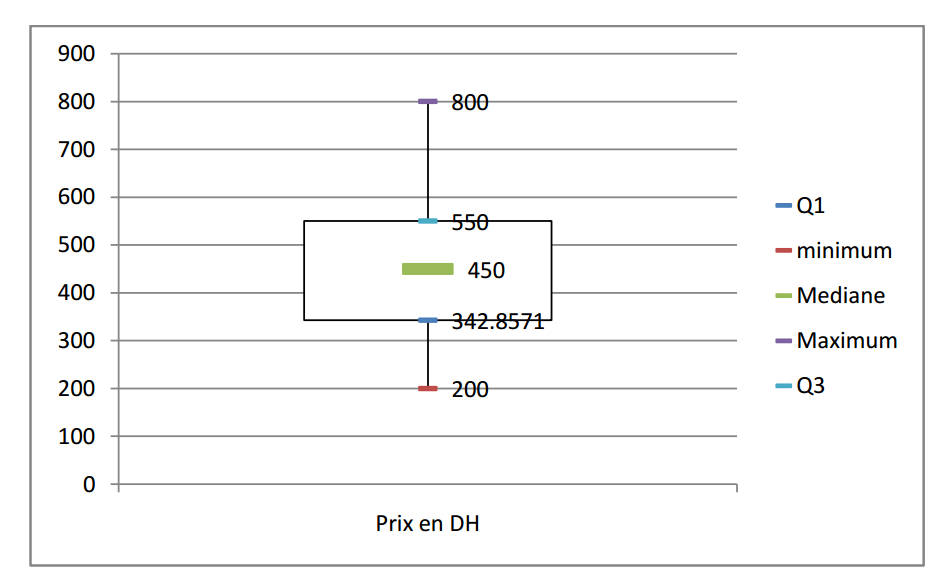
\includegraphics[width=0.6\textwidth]{images/probabilites/prob-017-002.png}\\[4pt]
{\small\itshape Exemple de boîte à moustaches (box-plot) : médiane, quartiles et extrêmes.}
\end{center}

\begin{center}

\includegraphics[width=0.6\textwidth]{images/probabilites/prob-017-003.png}\\[4pt]
{\small\itshape Polygone des fréquences cumulées et médiane graphique.}
\end{center}
\end{boitecorrige}

\subsection*{Exercice 10 - Régression linéaire \niveau{\moyen}}

\begin{boiteexercice}
On dispose de la série double suivante :
\[
\begin{array}{|c|c|c|c|c|c|}
\hline
X_i & 2 & 5 & 6 & 10 & 12 \\
\hline
Y_i & 83 & 70 & 70 & 54 & 49 \\
\hline
\end{array}
\]
\begin{enumerate}
  \item Calculer la covariance $\mathrm{Cov}(X,Y)$.
  \item Déterminer la droite de régression $Y = aX + b$.
  \item Calculer le coefficient de corrélation linéaire $r$ et le coefficient de détermination $R^2$. Commenter.
\end{enumerate}
\end{boiteexercice}

\begin{boitecorrige}
\textbf{1.} $n=5$. $\bar{X} = (2+5+6+10+12)/5 = 7$. $\bar{Y} = (83+70+70+54+49)/5 = 65{,}2$.
\[
\overline{XY} = \frac{1}{5}(2\times83+5\times70+6\times70+10\times54+12\times49) = \frac{2064}{5} = 412{,}8
\]
\[
\mathrm{Cov}(X,Y) = \overline{XY} - \bar{X}\bar{Y} = 412{,}8 - 7\times65{,}2 = 412{,}8 - 456{,}4 = \boxed{-43{,}6}
\]

\textbf{2.} $\mathrm{Var}(X) = \overline{X^2} - \bar{X}^2 = (4+25+36+100+144)/5 - 49 = 61{,}8-49 = 12{,}8$.
\[
a = \frac{\mathrm{Cov}(X,Y)}{\mathrm{Var}(X)} = \frac{-43{,}6}{12{,}8} \approx -3{,}41 \qquad b = \bar{Y} - a\bar{X} = 65{,}2 + 3{,}41\times7 \approx 89{,}1
\]
\[
\boxed{Y = -3{,}41X + 89{,}1}
\]

\textbf{3.} $\mathrm{Var}(Y) = \overline{Y^2}-\bar{Y}^2 = (6889+4900+4900+2916+2401)/5 - 65{,}2^2 = 4401{,}2 - 4251{,}04 = 150{,}16$.
\[
r = \frac{\mathrm{Cov}(X,Y)}{\sqrt{\mathrm{Var}(X)\cdot\mathrm{Var}(Y)}} = \frac{-43{,}6}{\sqrt{12{,}8\times150{,}16}} = \frac{-43{,}6}{\sqrt{1922}} \approx \frac{-43{,}6}{43{,}84} \approx \boxed{-0{,}995}
\]
$R^2 = r^2 \approx 0{,}990$. La corrélation est très fortement négative : quand $X$ augmente, $Y$ diminue quasi linéairement.
\end{boitecorrige}

\subsection*{Exercice 11 - Calculs de probabilités pour la loi normale \niveau{\moyen}}

\begin{boiteexercice}
Soit $X \sim \mathcal{N}(0,1)$.
\begin{enumerate}
  \item Calculer $P[X \leq 1{,}62]$, $P[X \geq -0{,}52]$, $P[-1 < X < 1]$.
  \item Trouver $u$ tel que $P[X \leq u] = 0{,}334$.
\end{enumerate}
\end{boiteexercice}

\begin{boitecorrige}
On note $\Phi$ la fonction de répartition de $\mathcal{N}(0,1)$ (table de Laplace-Gauss).

\textbf{1.}
\begin{itemize}[nosep]
  \item $P[X \leq 1{,}62] = \Phi(1{,}62) \approx \boxed{0{,}9474}$.
  \item $P[X \geq -0{,}52] = 1 - \Phi(-0{,}52) = \Phi(0{,}52) \approx \boxed{0{,}6985}$.
  \item $P[-1 < X < 1] = \Phi(1) - \Phi(-1) = 2\Phi(1) - 1 \approx 2\times0{,}8413-1 = \boxed{0{,}6827}$ (règle empirique : environ 68\% dans $[\mu\pm\sigma]$).
\end{itemize}

\textbf{2.} On cherche $u$ tel que $\Phi(u) = 0{,}334 < 0{,}5$ : $u < 0$.
\[
\Phi(u) = 0{,}334 \quad\Rightarrow\quad 1-\Phi(-u) = 0{,}334 \quad\Rightarrow\quad \Phi(-u) = 0{,}666
\]
Dans la table : $\Phi(0{,}43) \approx 0{,}6664$, donc $-u \approx 0{,}43$.
\[
\boxed{u \approx -0{,}43}
\]
\end{boitecorrige}

\subsection*{Exercice 12 - Densité de probabilité continue \niveau{\moyen}}

\begin{boiteexercice}
Soit $X$ une variable aléatoire continue dont la densité est :
\[
f(x) = \begin{cases} a(9x-3x^2) & 0 < x < 3 \\ 0 & \text{sinon} \end{cases}
\]
\begin{enumerate}
  \item Calculer la constante $a$.
  \item Calculer $P[X > 1]$ et $P[1/2 < X < 3/2]$.
  \item Donner la fonction de répartition $F(x)$.
  \item Calculer $\mathbb{E}(X)$ et $V(X)$.
\end{enumerate}
\end{boiteexercice}

\begin{boitecorrige}
\textbf{1.} Condition $\int_0^3 a(9x-3x^2)\,\mathrm{d}x = 1$ :
\[
a\left[\frac{9x^2}{2}-x^3\right]_0^3 = a\cdot\frac{27}{2} = 1 \quad\Rightarrow\quad \boxed{a = \frac{2}{27}}
\]

\textbf{2.}
\begin{align*}
P[X>1] &= \frac{2}{27}\int_1^3(9x-3x^2)\,\mathrm{d}x
= \frac{2}{27}\!\left[\frac{27}{2}-\frac{7}{2}\right] = \frac{2}{27}\cdot10 = \boxed{\frac{20}{27}}\\[6pt]
P\!\left[\tfrac{1}{2}<X<\tfrac{3}{2}\right] &= \frac{2}{27}\int_{1/2}^{3/2}(9x-3x^2)\,\mathrm{d}x
= \frac{2}{27}\cdot\frac{46}{8} = \boxed{\frac{23}{54}}
\end{align*}

\textbf{3.} Pour $0 \leq x \leq 3$ :
\[
F(x) = \frac{2}{27}\int_0^x(9t-3t^2)\,\d t
     = \frac{2}{27}\!\left[\frac{9t^2}{2}-t^3\right]_0^x
     = \frac{2}{27}\!\left(\frac{9x^2}{2}-x^3\right)
     = \frac{x^2(9-2x)}{27}
\]
$F(x)=0$ pour $x\leq0$, $F(x)=1$ pour $x\geq3$.

\textbf{4.}
\begin{align*}
\mathbb{E}(X) &= \frac{2}{27}\int_0^3 x(9x-3x^2)\,\mathrm{d}x = \frac{2}{27}\!\left[3x^3-\frac{3x^4}{4}\right]_0^3 = \frac{2}{27}\!\left(81-\frac{243}{4}\right) = \frac{3}{2}
\end{align*}
\begin{align*}
\mathbb{E}(X^2) &= \frac{2}{27}\int_0^3 x^2(9x-3x^2)\,\mathrm{d}x = \frac{2}{27}\!\left[\frac{9x^4}{4}-\frac{3x^5}{5}\right]_0^3\\
&= \frac{2}{27}\!\left(\frac{729}{4}-\frac{729}{5}\right) = \frac{2}{27}\cdot\frac{729}{20} = \frac{27}{10}
\end{align*}
\[
V(X) = \frac{27}{10} - \left(\frac{3}{2}\right)^2 = \frac{27}{10} - \frac{9}{4} = \frac{54-45}{20} = \boxed{\frac{9}{20}}
\]
\end{boitecorrige}

\subsection*{Exercice 13 - Loi de Poisson et somme de variables \niveau{\difficile}}

\begin{boiteexercice}
On dit que $X$ suit une loi de Poisson de paramètre $\lambda > 0$ (noté $X \sim \mathcal{P}(\lambda)$) si :
\[
\mathbb{P}(X=k) = e^{-\lambda}\frac{\lambda^k}{k!}, \quad k\in\mathbb{N}
\]
\begin{enumerate}
  \item Rappeler $\mathbb{E}(X)$ et $V(X)$ pour $X\sim\mathcal{P}(\lambda)$.
  \item Montrer que si $X_1\sim\mathcal{P}(\lambda_1)$ et $X_2\sim\mathcal{P}(\lambda_2)$ sont indépendantes, alors $X_1+X_2\sim\mathcal{P}(\lambda_1+\lambda_2)$.
  \item Un centre d'appels reçoit en moyenne 3 appels par minute. Calculer la probabilité de recevoir exactement 5 appels en une minute, puis moins de 2 appels.
\end{enumerate}
\end{boiteexercice}

\begin{boitecorrige}
\textbf{1.} Pour $X\sim\mathcal{P}(\lambda)$ : $\mathbb{E}(X) = \lambda$ et $V(X) = \lambda$.

\textbf{2.} Calculons $\mathbb{P}(X_1+X_2=n)$ par la formule de convolution :
\[
\mathbb{P}(X_1+X_2=n) = \sum_{k=0}^n \mathbb{P}(X_1=k)\mathbb{P}(X_2=n-k) = \sum_{k=0}^n e^{-\lambda_1}\frac{\lambda_1^k}{k!}\cdot e^{-\lambda_2}\frac{\lambda_2^{n-k}}{(n-k)!}
\]
\[
= e^{-(\lambda_1+\lambda_2)}\frac{1}{n!}\sum_{k=0}^n\binom{n}{k}\lambda_1^k\lambda_2^{n-k} = e^{-(\lambda_1+\lambda_2)}\frac{(\lambda_1+\lambda_2)^n}{n!}
\]
C'est bien $\mathcal{P}(\lambda_1+\lambda_2)$.

\textbf{3.} $X\sim\mathcal{P}(3)$.
\[
\mathbb{P}(X=5) = e^{-3}\frac{3^5}{5!} = e^{-3}\frac{243}{120} \approx 0{,}0498\times2{,}025 \approx \boxed{0{,}101}
\]
\[
\mathbb{P}(X<2) = \mathbb{P}(X=0)+\mathbb{P}(X=1) = e^{-3}(1+3) = 4e^{-3} \approx 4\times0{,}0498 \approx \boxed{0{,}199}
\]
\end{boitecorrige}

\subsection*{Exercice 14 - Loi binomiale et approximation \niveau{\moyen}}

\begin{boiteexercice}
Un QCM comporte 20 questions, chacune avec 4 réponses dont une seule est correcte. Un étudiant répond au hasard à chaque question. Soit $X$ le nombre de bonnes réponses.
\begin{enumerate}
  \item Donner la loi de $X$, son espérance et sa variance.
  \item Calculer la probabilité d'obtenir exactement 5 bonnes réponses.
  \item Calculer la probabilité d'obtenir plus de 8 bonnes réponses.
  \item En utilisant l'approximation normale, recalculer la probabilité de la question 3.
\end{enumerate}
\end{boiteexercice}

\begin{boitecorrige}
\textbf{1.} Chaque question a probabilité $p = 1/4$ d'être correcte, indépendamment des autres. Donc $X \sim \mathcal{B}(20, 1/4)$.
\[
\mathbb{E}(X) = np = 20\times\frac{1}{4} = 5 \qquad V(X) = np(1-p) = 20\times\frac{1}{4}\times\frac{3}{4} = \frac{15}{4} = 3{,}75
\]

\textbf{2.}
\[
\mathbb{P}(X=5) = \binom{20}{5}\!\left(\frac{1}{4}\right)^5\!\left(\frac{3}{4}\right)^{15} = 15504\times\frac{1}{1024}\times\frac{3^{15}}{4^{15}}
\]
$3^{15} = 14\,348\,907$, $4^{15} = 2^{30} \approx 1{,}074\times10^9$.
\[
\mathbb{P}(X=5) \approx 15504\times\frac{14\,348\,907}{1024\times1{,}074\times10^9} \approx \boxed{0{,}202}
\]

\textbf{3.} $\mathbb{P}(X>8) = 1-\mathbb{P}(X\leq8) = 1-\sum_{k=0}^8\binom{20}{k}(1/4)^k(3/4)^{20-k} \approx \boxed{0{,}041}$.

\textbf{4.} Approximation normale : $\mu=5$, $\sigma=\sqrt{3{,}75}\approx1{,}936$. Avec correction de continuité :
\[
\mathbb{P}(X>8) \approx \mathbb{P}\!\left(Z > \frac{8{,}5-5}{1{,}936}\right) = \mathbb{P}(Z > 1{,}81) = 1-\Phi(1{,}81) \approx 1-0{,}9649 \approx \boxed{0{,}035}
\]
\end{boitecorrige}


% ================================================================
\section{Examens corrigés}
% ================================================================

\subsection*{Examen 2021-2022 - Dénombrement et Calcul de Probabilité}

\subsubsection*{Exercice 1 (6 pts) - Fiabilité d'avions \niveau{\moyen}}

\begin{boiteexercice}
$A$ et $B$ sont deux avions ayant respectivement 4 et 2 moteurs. Les moteurs sont supposés indépendants et ont chacun une probabilité $p$ de tomber en panne. Chaque avion arrive à destination si \textit{moins de la moitié} de ses moteurs tombe en panne. Quel avion choisissez-vous ? (discuter en fonction de $p$).
\end{boiteexercice}

\begin{boitecorrige}
Soit $X_A \sim \mathcal{B}(4,p)$ le nombre de moteurs en panne de $A$, et $X_B \sim \mathcal{B}(2,p)$ celui de $B$.

\textbf{Probabilité d'arrivée de $A$} (moins de 2 pannes sur 4) :
\begin{align*}
P_A &= \mathbb{P}(X_A < 2) = \mathbb{P}(X_A=0) + \mathbb{P}(X_A=1)\\
    &= (1-p)^4 + 4p(1-p)^3.
\end{align*}

\textbf{Probabilité d'arrivée de $B$} (moins de 1 panne sur 2) :
\[
P_B = \mathbb{P}(X_B=0) = (1-p)^2.
\]

On compare $P_A$ et $P_B$. Posons $q = 1-p$ :
\[
P_A - P_B = q^4 + 4pq^3 - q^2 = q^2\!\left(q^2 + 4pq - 1\right).
\]
Puisque $q^2 \geq 0$, le signe dépend de $f(q) = q^2 + 4pq - 1 = q^2 + 4(1-q)q - 1 = 4q - 3q^2 - 1$.

$f(q) = -(3q^2 - 4q + 1) = -(3q-1)(q-1)$.

$f(q) \geq 0 \iff (3q-1)(q-1) \leq 0 \iff q \in [1/3, 1]$, soit $p \leq 2/3$.

\textbf{Conclusion :}
\begin{itemize}[nosep]
  \item Si $p < 2/3$ (moteurs assez fiables) : $P_A > P_B$ $\Rightarrow$ choisir l'avion $A$ (4 moteurs).
  \item Si $p > 2/3$ (moteurs très peu fiables) : $P_A < P_B$ $\Rightarrow$ choisir l'avion $B$ (2 moteurs).
  \item Si $p = 2/3$ : les deux avions ont la même probabilité d'arriver.
\end{itemize}
\end{boitecorrige}

\subsubsection*{Exercice 2 (8 pts) - Numéro de téléphone aléatoire \niveau{\moyen}}

\begin{boiteexercice}
On compose au hasard un numéro de téléphone à 8 chiffres (chaque chiffre est choisi uniformément dans $\{0,1,\ldots,9\}$, indépendamment des autres). Quelle est la probabilité pour que :
\begin{enumerate}
  \item Tous les chiffres du numéro soient distincts ?
  \item Le produit des chiffres soit divisible par 2 ?
  \item Les chiffres forment une suite strictement croissante ?
  \item Les chiffres forment une suite croissante au sens large ?
\end{enumerate}
\end{boiteexercice}

\begin{boitecorrige}
L'espace de probabilité est $\Omega = \{0,\ldots,9\}^8$, avec $|\Omega| = 10^8$ résultats équiprobables.

\textbf{1. Tous les chiffres distincts.}
Le nombre de 8-uplets de chiffres distincts est $A_{10}^8 = 10 \times 9 \times 8 \times \cdots \times 3$.
\[
P_1 = \frac{10!/(10-8)!}{10^8} = \frac{10!}{2!\cdot 10^8}
     = \frac{3\,628\,800}{200\times 10^6} \approx \boxed{0{,}0181}.
\]

\textbf{2. Produit divisible par 2.}
Le produit est divisible par 2 sauf si tous les chiffres sont impairs. Il y a 5 chiffres impairs parmi 10.
\[
P_2 = 1 - \left(\frac{5}{10}\right)^8 = 1 - \frac{1}{256} \approx \boxed{0{,}996}.
\]

\textbf{3. Suite strictement croissante.}
Une suite strictement croissante de 8 chiffres distincts de $\{0,\ldots,9\}$ correspond à un sous-ensemble à 8 éléments, ordonné de façon unique. Il y a $\binom{10}{8} = 45$ tels sous-ensembles.
\[
P_3 = \frac{45}{10^8} \approx \boxed{4{,}5 \times 10^{-7}}.
\]

\textbf{4. Suite croissante au sens large.}
C'est le nombre de 8-uplets $(d_1,\ldots,d_8)$ avec $0\leq d_1\leq d_2\leq\cdots\leq d_8\leq 9$. Par le principe des étoiles et barres (combinaisons avec répétition) :
\[
\binom{10+8-1}{8} = \binom{17}{8} = 24\,310.
\]
\[
P_4 = \frac{24\,310}{10^8} \approx \boxed{2{,}43 \times 10^{-4}}.
\]
\end{boitecorrige}

\subsubsection*{Exercice 3 (8 pts) - Loi de Poisson \niveau{\difficile}}

\begin{boiteexercice}
Soit $X$ une variable aléatoire suivant une loi de Poisson de paramètre $\lambda > 0$ : $\mathbb{P}(X=k) = \dfrac{\lambda^k}{k!}e^{-\lambda}$, pour $k \in \mathbb{N}$.
\begin{enumerate}
  \item Montrer que $\mathbb{P}(X=k+1) = \dfrac{\lambda}{k+1}\,\mathbb{P}(X=k)$.
  \item Montrer que $\mathbb{E}(X) = \lambda$ et calculer $\mathrm{Var}(X)$.
  \item Montrer que si $X_1$ et $X_2$ sont deux v.a.\ indépendantes suivant respectivement $\mathcal{P}(\lambda_1)$ et $\mathcal{P}(\lambda_2)$, alors $X_1+X_2 \sim \mathcal{P}(\lambda_1+\lambda_2)$.
\end{enumerate}
\end{boiteexercice}

\begin{boitecorrige}
\textbf{1.}
\[
\mathbb{P}(X=k+1) = \frac{\lambda^{k+1}}{(k+1)!}e^{-\lambda}
= \frac{\lambda}{k+1}\cdot\frac{\lambda^k}{k!}e^{-\lambda}
= \frac{\lambda}{k+1}\,\mathbb{P}(X=k). \quad \square
\]

\textbf{2. Espérance.}
\[
\mathbb{E}(X) = \sum_{k=0}^{\infty} k\,\frac{\lambda^k}{k!}e^{-\lambda}
= \lambda\,e^{-\lambda}\sum_{k=1}^{\infty}\frac{\lambda^{k-1}}{(k-1)!}
= \lambda\,e^{-\lambda}\,e^{\lambda} = \boxed{\lambda}.
\]

\textbf{Variance.} On calcule $\mathbb{E}(X(X-1))$ :
\[
\mathbb{E}(X(X-1)) = \lambda^2 e^{-\lambda}\sum_{k=2}^{\infty}\frac{\lambda^{k-2}}{(k-2)!} = \lambda^2.
\]
Donc $\mathbb{E}(X^2) = \lambda^2+\lambda$, et :
\[
\mathrm{Var}(X) = \mathbb{E}(X^2)-[\mathbb{E}(X)]^2 = \lambda^2+\lambda-\lambda^2 = \boxed{\lambda}.
\]

\textbf{3. Stabilité par convolution.}
En utilisant la fonction génératrice des probabilités $G_X(t) = e^{\lambda(t-1)}$ :
\[
G_{X_1+X_2}(t) = G_{X_1}(t)\,G_{X_2}(t) = e^{\lambda_1(t-1)}\,e^{\lambda_2(t-1)}
= e^{(\lambda_1+\lambda_2)(t-1)},
\]
qui est la fgp d'une loi $\mathcal{P}(\lambda_1+\lambda_2)$. Donc $X_1+X_2\sim\mathcal{P}(\lambda_1+\lambda_2)$. $\square$
\end{boitecorrige}

\newpage
% ================================================================
\subsection*{Examen 2022-2023 - Dénombrement et Calcul de Probabilité}

\subsubsection*{Exercice 1 (5 pts) - Couple de variables aléatoires uniforme \niveau{\moyen}}

\begin{boiteexercice}
Soit $(X,Y)$ un couple de variables aléatoires suivant une loi uniforme sur $\{0,1,\ldots,n\}^2$.
\begin{enumerate}
  \item Déterminer la loi de $X$, la loi de $Y$, et la loi de $X+Y$.
  \item $X$ et $Y$ sont-elles indépendantes ?
\end{enumerate}
\end{boiteexercice}

\begin{boitecorrige}
La loi conjointe est $\mathbb{P}(X=x, Y=y) = \dfrac{1}{(n+1)^2}$ pour tout $(x,y)\in\{0,\ldots,n\}^2$.

\textbf{1. Loi marginale de $X$ :}
\[
\mathbb{P}(X=x) = \sum_{y=0}^n \mathbb{P}(X=x,Y=y) = \frac{n+1}{(n+1)^2} = \frac{1}{n+1}, \quad x\in\{0,\ldots,n\}.
\]
$X$ suit une loi uniforme sur $\{0,\ldots,n\}$. De même $Y\sim\mathcal{U}(\{0,\ldots,n\})$.

\textbf{Loi de $X+Y$ :} Pour $k\in\{0,\ldots,2n\}$, les paires $(x,y)$ avec $x+y=k$ et $0\leq x,y\leq n$ sont au nombre de $k+1$ si $k\leq n$, et $2n-k+1$ si $k>n$. Donc :
\[
\mathbb{P}(X+Y=k) = \frac{\min(k,2n-k)+1}{(n+1)^2}.
\]

\textbf{2. Indépendance :}
$\mathbb{P}(X=x)\cdot\mathbb{P}(Y=y) = \dfrac{1}{(n+1)^2} = \mathbb{P}(X=x,Y=y)$.

Donc $X$ et $Y$ \textbf{sont indépendantes}.
\end{boitecorrige}

\subsubsection*{Exercice 2 (5 pts) - Loi log-normale \niveau{\difficile}}

\begin{boiteexercice}
Une variable aléatoire $X$ suit une loi log-normale de paramètres $\mu$ et $\sigma^2$ si $Y = \ln X$ suit une loi $\mathcal{N}(\mu, \sigma^2)$. Sa densité est :
\[
f_X(x) = \frac{1}{x\sigma\sqrt{2\pi}}\exp\!\left(-\frac{(\ln x - \mu)^2}{2\sigma^2}\right), \quad x > 0.
\]
Montrer que $\mathbb{E}(X) = e^{\mu+\sigma^2/2}$ et $\mathrm{Var}(X) = (e^{\sigma^2}-1)\,e^{2\mu+\sigma^2}$.
\end{boiteexercice}

\begin{boitecorrige}
\textbf{Espérance.} Par le changement de variable $y = \ln x$ (soit $x = e^y$, $dx = e^y\,dy$) :
\[
\mathbb{E}(X) = \int_0^\infty x\,f_X(x)\,dx
= \int_{-\infty}^{+\infty} e^y \cdot \frac{1}{\sigma\sqrt{2\pi}}e^{-(y-\mu)^2/(2\sigma^2)}\,dy.
\]
On complète le carré dans l'exposant :
\[
y - \frac{(y-\mu)^2}{2\sigma^2} = -\frac{(y-(\mu+\sigma^2))^2}{2\sigma^2} + \mu + \frac{\sigma^2}{2}.
\]
Ainsi :
\[
\mathbb{E}(X) = e^{\mu+\sigma^2/2}\int_{-\infty}^{+\infty}\frac{1}{\sigma\sqrt{2\pi}}e^{-(y-\mu-\sigma^2)^2/(2\sigma^2)}\,dy = \boxed{e^{\mu+\sigma^2/2}}.
\]

\textbf{Variance.} De même :
\[
\mathbb{E}(X^2) = \int_0^\infty x^2 f_X(x)\,dx = e^{2\mu+2\sigma^2}
\]
(en remplaçant $y$ par $2y$ dans le calcul précédent, soit en appliquant la formule avec $\mu' = \mu$, $\sigma'^2 = \sigma^2$ et $e^{2y}$). On obtient $\mathbb{E}(X^2) = e^{2\mu+2\sigma^2}$.

\[
\mathrm{Var}(X) = \mathbb{E}(X^2) - [\mathbb{E}(X)]^2 = e^{2\mu+2\sigma^2} - e^{2\mu+\sigma^2}
= e^{2\mu+\sigma^2}(e^{\sigma^2}-1). \quad \square
\]
\end{boitecorrige}

\subsubsection*{Exercice 3 (5 pts) - Vrai ou Faux \niveau{\facile}}

\begin{boiteexercice}
Répondre par Vrai ou Faux à chaque affirmation (une rature ou une surcharge équivaut à la note 0) :
\begin{enumerate}
  \item Tout sous-ensemble de $\mathbb{R}$ est soit fini soit dénombrable.
  \item Pour trois événements quelconques $A,B,C$ : $\mathbb{P}(A\cup B\cup C)=\mathbb{P}(A)+\mathbb{P}(B)+\mathbb{P}(C)-\mathbb{P}(A\cap B)-\mathbb{P}(A\cap C)-\mathbb{P}(B\cap C)+\mathbb{P}(A\cap B\cap C)$.
  \item Si $\mathrm{Card}(E)=\mathrm{Card}(F)$, le nombre de permutations de $F$ égale le nombre de bijections $E\to F$.
  \item Deux variables aléatoires continues centrées sont toujours indépendantes.
  \item Pour deux événements $A$ et $B$ indépendants, $\mathrm{Card}(A\cup B)=\mathrm{Card}(A)+\mathrm{Card}(B)$.
  \item Si $X\sim\mathcal{N}(\mu,\sigma^2)$, alors $\frac{X-\mu}{\sigma}\sim\mathcal{N}(0,1)$.
  \item Deux variables aléatoires indépendantes sont non corrélées.
  \item Si $X_1\sim\mathcal{P}(\lambda_1)$ et $X_2\sim\mathcal{P}(\lambda_2)$ sont indépendantes, alors $X_1+X_2\sim\mathcal{P}(\lambda_1+\lambda_2)$.
  \item Si $X$ et $Y$ sont indépendantes, alors $F_{XY}(x,y)=F_X(x)+F_Y(y)$.
  \item La variance d'une variable aléatoire centrée réduite est égale à son moment d'ordre 2.
  \item Pour $X$ géométrique de paramètre $\lambda$ : $\mathbb{E}(X)=\lambda^{-1}$ et $\mathrm{Var}(X)=\lambda^{-2}(1-\lambda)$.
  \item La loi $\mathcal{B}(n,p)$ peut être approchée par une loi de Poisson si $n\geq 30$.
  \item Si $X$ suit une loi de Cauchy centrée, alors $\mathbb{E}(X)$ existe.
\end{enumerate}
\end{boiteexercice}

\begin{boitecorrige}
\begin{center}
\begin{tabular}{|c|c|c|c|c|c|c|c|c|c|c|c|c|c|}
\hline
Q & 1 & 2 & 3 & 4 & 5 & 6 & 7 & 8 & 9 & 10 & 11 & 12 & 13 \\
\hline
R & F & V & V & F & F & V & V & V & F & V & F & V & F \\
\hline
\end{tabular}
\end{center}

\begin{enumerate}
  \item \textbf{Faux} : $[0,1]$ est un sous-ensemble de $\mathbb{R}$ qui n'est ni fini ni dénombrable (il est indénombrable, par l'argument diagonal de Cantor).
  \item \textbf{Vrai} : c'est la formule d'inclusion-exclusion (avec un signe $+$ devant le terme triple).
  \item \textbf{Vrai} : si $|E|=|F|=n$, il y a $n!$ permutations de $F$ et $n!$ bijections $E\to F$.
  \item \textbf{Faux} : l'indépendance est une condition bien plus forte que d'être centrée. Exemple : $X\sim\mathcal{N}(0,1)$ et $Y=X^2$ sont non corrélées (centrées) mais dépendantes.
  \item \textbf{Faux} : l'indépendance est une notion probabiliste, pas ensembliste ; le cardinal d'une union n'est pas lié à l'indépendance.
  \item \textbf{Vrai} : par définition de la loi normale centrée réduite.
  \item \textbf{Vrai} : l'indépendance implique la non-corrélation (la réciproque est fausse en général).
  \item \textbf{Vrai} : propriété de stabilité de la loi de Poisson (démontrée en exercice 3 de l'examen 2021-2022).
  \item \textbf{Faux} : si $X$ et $Y$ sont indépendantes, $F_{XY}(x,y)=F_X(x)\cdot F_Y(y)$ (produit, non somme).
  \item \textbf{Vrai} : une v.a.\ centrée réduite a $\mathbb{E}(X)=0$, donc $\mathrm{Var}(X)=\mathbb{E}(X^2)-0=\mathbb{E}(X^2)$.
  \item \textbf{Faux} : pour la loi géométrique de paramètre $p$ (proba de succès), $\mathbb{E}(X)=1/p$ et $\mathrm{Var}(X)=(1-p)/p^2$, soit $\lambda^{-2}(1-\lambda)$ avec $\lambda=p$ ; mais la formule avec $\lambda^{-1}$ pour la variance est incorrecte.
  \item \textbf{Vrai} (approximation de Poisson) : $\mathcal{B}(n,p)$ est bien approchée par $\mathcal{P}(np)$ quand $n$ est grand et $p$ petit ($n\geq 30$, $p\leq 0{,}1$ sont des critères courants).
  \item \textbf{Faux} : la loi de Cauchy standard n'a pas d'espérance (l'intégrale $\int |x|f(x)\,dx$ diverge).
\end{enumerate}
\end{boitecorrige}

\ifdefined\inMainDoc\else\end{document}\fi
